\documentclass[11pt]{article}
\usepackage[margin=1in]{geometry}
\usepackage[T1]{fontenc}
\usepackage{lmodern,microtype,amsmath,amssymb,amsthm,booktabs,graphicx,enumitem}
\usepackage[round]{natbib}
\usepackage[hidelinks]{hyperref}
\usepackage{float}
\graphicspath{{../figures/}}
\newtheorem{theorem}{Theorem}
\newtheorem{proposition}[theorem]{Proposition}
\newtheorem{corollary}[theorem]{Corollary}
\newtheorem{lemma}[theorem]{Lemma}
\theoremstyle{definition}\newtheorem{definition}[theorem]{Definition}
\newcommand{\E}{\mathbb{E}}
\newcommand{\R}{\mathbb{R}}
\newcommand{\1}{\mathbf{1}}
\newcommand{\simplex}{\Delta_M}
\newcommand{\bad}{\mathcal B}
\newcommand{\nearset}{\mathcal A}
\newcommand{\gap}{g}
\newcommand{\Gam}{\Gamma}
\newcommand{\eps}{\varepsilon}
\newcommand{\supp}{\operatorname{supp}}
\newcommand{\argmax}{\operatorname*{arg\,max}}
\newcommand{\argmin}{\operatorname*{arg\,min}}
\newcommand{\KL}{\operatorname{KL}}
\newcommand{\kl}{\operatorname{kl}}
\title{Which Environments Teach Cooperation?\\Diagnostic Exposure for Compatible Self-Play}
\author{Anonymous research draft}
\date{September 2026}
\begin{document}
\maketitle
\begin{abstract}
Independently trained self-play policies can be individually competent yet mutually incompatible. We study which distributions over training environments make \emph{all approximately optimal self-play solutions} compatible on a specified target task family. For finite policy classes, a pair-exclusion margin characterizes this property. In a two-role assignment game with restricted observations, we derive an exact balanced-coverage formula: incompatibility is possible precisely when a harmful set of convention errors can be divided between two learners without exceeding either learner's self-play error budget. This yields an observability obstruction, an exact diagnostic-dilution law, and a distinction between teaching compatible behavior and identifying a unique policy. For general finite classes, a sequence of linear programs attains half the optimal margin, and a three-policy example makes the factor tight for this surrogate. We also give a closed-form, sharp certificate over rectangular return intervals that remains valid after data-dependent curriculum selection, together with a restricted calibration lower bound. CPU-only validation includes 300 structured instances, 400 interval witnesses, and 2,016 learned-policy runs. Diagnostic weighting improves the guaranteed optimization tolerance but does not uniformly maximize empirical cross-play: simpler weighting sometimes performs better, and independent-action policy gradient often fails to reach the required near-optimal set. The results isolate environmental information, statistical uncertainty, and optimization as distinct requirements for transferable cooperation.
\end{abstract}

\section{Introduction}
Two independently trained systems may each solve a cooperative task in self-play while failing when paired. Self-play can select different conventions, including incompatible assignments of roles, resources, or actions. Other-Play uses known symmetries to reduce specialized conventions \citep{hu2020}; subsequent formal work explains why incompatible maximizing policies and tie-breaking remain important \citep{treutlein2021}. Recent environment-distribution approaches provide a different route: learning to cooperate across many tasks rather than specializing to one \citep{jha2025,you2025}.

This paper asks a narrower question than whether diversity helps empirically: \emph{which environmental distinctions, and how much exposure to them, suffice to exclude harmful pairs of approximately optimal self-play policies?} Task count is not enough. Many changes can leave competing conventions equally effective. Even a useful task may receive too little probability to separate these conventions at a learner's optimization accuracy. Conversely, forcing a unique policy may unnecessarily remove distinct solutions that already cooperate.

Consider three conventions with source self-play returns $(1,.8,1)$ and $(1,1,.8)$ on two diagnostic environments. All mismatched target pairs fail. Equal training on these two sources gives a compatibility margin of $.1$. Adding eighteen neutral sources, each with return $(1,1,1)$, and sampling uniformly reduces the margin to $.01$. A $.02$-optimal learner must choose the first convention before dilution, but may choose any convention afterward. The best exact solution is unchanged; the set of approximate solutions is not. This is a statement about \emph{exposure allocation}, not a claim that enlarging the set of available curricula reduces its optimum.

We develop three linked results. First, a structured assignment game turns compatibility into a balanced covering problem: two learners can distribute errors across different contexts, so controlling a single learner's disagreement with a reference can miss a factor of two. Second, a general finite-class curriculum optimizer achieves a sharp factor-two guarantee for a pair-sum surrogate. Third, a rectangular-interval certificate makes the resulting guarantee robust to finite evaluation data and adaptive choice of curriculum weights. All proofs are constructive. Exact oracles and deliberate assumption violations accompany the learned experiments.

The scope is intentionally limited. Policies are from a specified class; curricula are stationary environment distributions; target compatibility is given or bounded; learners are only covered when their \emph{global} self-play gap is sufficiently small. We do not prove convergence of arbitrary reinforcement-learning algorithms, unrestricted transfer to unseen observations, or cooperation with humans and large language models. In fact, a local-optimization obstruction and a negative policy-gradient experiment show why these restrictions matter.

\section{Related work and the distinction from teaching a target}
\paragraph{Coordination and environment diversity.}
Other-Play modifies self-play using known symmetries \citep{hu2020}. Label-free coordination makes the role of incompatible maximizers explicit \citep{treutlein2021}. Cross-Environment Cooperation trains across procedural environments and evaluates general cooperative behavior \citep{jha2025}. Automatic curriculum design for human--AI coordination jointly selects environments and co-players using coordination-related utility \citep{you2025}. COLE also uses a graph view of cooperative incompatibility in population learning \citep{li2023}. Thus neither incompatibility graphs nor environment selection are new in isolation. Our object is the \emph{entire near-optimal self-play set} induced by a stationary curriculum, with a guarantee on every pair in that set.

\paragraph{Machine teaching and version-space diameter.}
Selecting informative examples and reducing teaching to covering are established ideas; machine teaching for inverse reinforcement learning targets reward-equivalence classes through informative demonstrations \citep{brown2019}. Diameter-based active learning studies how queries reduce disagreement within a hypothesis set \citep{tosh2017}. Our finite-class formulation has a genuine connection to these ideas and should not be interpreted as independent invention of version-space reasoning. Its distinguishing ingredients are self-play \emph{reward gaps} rather than label consistency, a target pairwise cooperation relation that need not identify one hypothesis, an exact two-learner error-budget partition in the assignment model, and a sharp uncertainty certificate for curriculum-selected score sets. We do not establish a separation from every possible general machine-teaching formalism.

\paragraph{What the experiments compare.}
The baseline curricula below are controlled selection rules, not implementations of Other-Play, CEC, COLE, or multi-agent UED. Their role is to test diagnostic exposure, not establish state-of-the-art performance. The synthetic environment is small enough to distinguish environmental insufficiency from statistical and optimization failure exactly.

\section{Finite-policy curriculum design}
Let $\Pi=\{\pi_1,\ldots,\pi_K\}$ be a finite class of role-conditioned policies and let $e\in[M]$ index admissible training environments. Two copies of one policy constitute self-play; role conditioning permits them to take different actions. Define
\begin{equation}
 A_{ei}=J_e(\pi_i,\pi_i)\in[0,1],\quad
 S_i(\mu)=\sum_e\mu_e A_{ei},\quad
 g_i(\mu)=\max_k S_k(\mu)-S_i(\mu),
 \label{eq:scores}
\end{equation}
where $\mu\in\simplex$ is a stationary curriculum. For a tolerance $\eta\geq0$, let
\begin{equation}
 \nearset_\eta(\mu)=\{i:g_i(\mu)\leq\eta\}.
\end{equation}
Different training seeds may select different members of this set. This model constrains their final quality, not their learning trajectories.

Let $T_{ij}\in[0,1]$ be target cross-play return, already averaged over a specified target distribution and with $i,j$ assigned to the two roles. For a target threshold $\tau$, define
\begin{equation}
 \bad=\{(i,j):T_{ij}<\tau\},\qquad
 \Gam_A(\mu;\bad)=\min_{(i,j)\in\bad}\max\{g_i(\mu),g_j(\mu)\}.
 \label{eq:margin}
\end{equation}
When $\bad$ is empty the margin is $+\infty$. Diagonal bad pairs are allowed. An asymmetric target is handled by including both role orderings; identical unordered constraints may be merged computationally.

\begin{lemma}[Exact pair exclusion]\label{lem:margin}
For a finite class, every pair in $\nearset_\eta(\mu)$ has target return at least $\tau$ if and only if $\Gam_A(\mu;\bad)>\eta$.
\end{lemma}
\begin{proof}
A bad pair survives precisely when both gaps are at most $\eta$, equivalently when their maximum is at most $\eta$. Taking the minimum over bad pairs gives the equivalence. The strict inequality is necessary because boundary policies belong to $\nearset_\eta$.
\end{proof}
This elementary lemma is an organizing device, not the main technical claim. In graph language, the excluded policies must form a vertex cover of the bad-pair graph. There may remain many mutually compatible policies.

\paragraph{Access and generalization.}
The teacher initially has the return table and the target relation; Section~\ref{sec:statistics} replaces exact source values by intervals and also permits an uncertain target relation. Evaluating all $K$ policies can be expensive: the algorithms are polynomial in an \emph{enumerated} class, not in a compact neural representation. The target distribution is specified separately from training, rather than claimed to be arbitrary out of distribution.

\section{An exact diagnostic-coverage theory for assignment}
\label{sec:assignment}
\subsection{A fixed reward rule and restricted observations}
There are $d$ public contexts, two roles, and two workstations. A deterministic policy is a convention vector $b\in\{0,1\}^d$. In context $j$, role 0 chooses station $b_j$ and role 1 chooses station $1-b_j$. Thus two copies never collide; policies $b,c$ collide exactly on coordinates where $b_j\ne c_j$.

A fixed hidden preferred assignment $\theta_j$ describes relative processing capability. In source mode $e$, context $j$ occurs with probability $W_{ej}$ and the wrong coordinated assignment has extra normalized completion cost $\Delta_{ej}\in[0,1]$. The mode is not part of the policy observation. The common reward is a fixed normalized completion-cost function, with collision return zero. For instance, coordinated total costs $2s$ and $2s(1+\Delta_{ej})$ with reward $2-C/(2s)$ give returns $1$ and $1-\Delta_{ej}$. Varying $s>0$ changes physical scale without changing diagnostic information. This is a contextual one-step assignment game, not a manipulation simulator.

Set $D_{ej}=W_{ej}\Delta_{ej}$, with $D\geq0$ and $\sum_jD_{ej}\leq1$. On target tasks, coordinated costs are balanced and contexts follow $q\in\Delta_d$. Therefore
\begin{equation}
 A_e(b)=1-\sum_jD_{ej}\1\{b_j\ne\theta_j\},\qquad
 T(b,c)=1-\sum_jq_j\1\{b_j\ne c_j\}.
 \label{eq:assignment}
\end{equation}
The preference is shared across source modes, and the class uses the same convention for a context in all modes. These are substantive restrictions: observable source labels would permit different source and target behavior. A common source baseline other than 1 leaves every gap unchanged and will be used for noisy training.

Define the diagnostic exposure $a_j=\sum_e\mu_eD_{ej}$. Relabeling $b$ by $b\oplus\theta$ permits $\theta=0$ in the analysis; curriculum construction from $D$ does not require the preference bits themselves. For $U\subseteq[d]$, write $a(U)=\sum_{j\in U}a_j$ and $q(U)=\sum_{j\in U}q_j$. The target threshold is $\tau=1-\eps$, where $0\leq\eps<1$.

\subsection{Harmful mistakes may be split between learners}
\begin{theorem}[Balanced diagnostic coverage]\label{thm:balanced}
For the assignment family in~\eqref{eq:assignment}, the exact compatibility margin is
\begin{equation}
 \Gam(a;q,\eps)=
 \min_{U:q(U)>\eps}\ \min_{V\subseteq U}
 \max\{a(V),a(U\setminus V)\}.
 \label{eq:balanced}
\end{equation}
Consequently, if
\begin{equation}
 \kappa(a;q,\eps)=\min_{U:q(U)>\eps}a(U),
\end{equation}
then $\kappa/2\leq\Gam\leq\kappa$, and both constants are sharp over this family. Equivalently, incompatibility among $\eta$-optimal policies occurs precisely when there are disjoint sets $V,Z$ with
\begin{equation}
 q(V\cup Z)>\eps,\qquad a(V)\leq\eta,\qquad a(Z)\leq\eta.
 \label{eq:two-budget}
\end{equation}
\end{theorem}
\noindent\emph{Proof idea.} A policy's gap is the exposure of its wrong coordinates. A bad pair can share some wrong coordinates, but deleting their common mistakes preserves disagreement and only decreases both gaps. The remaining disjoint errors partition a harmful set. Conversely, every such partition specifies an actual pair of policies. Full details and sharp examples appear in Appendix~\ref{app:balanced}.

The distinction from reference identification is concrete. With two coordinates, exposures $(s,s)$, target weights $(1/2,1/2)$, and $\eps=3/4$, each learner can make one different mistake at gap $s$. Each is close to the reference on half the contexts, but together they disagree everywhere. The total harmful-set exposure is $2s$, while the true margin is only $s$.

Equation~\eqref{eq:balanced} also permits useful ambiguity. For $d=6$, uniform exposure $a_j=.4/6$, and $\eps=.413$, the margin is $2(.4/6)$. At tolerance $.8\Gam$, the reference and all six one-error conventions survive; any two disagree on at most $2/6<.413$ of target contexts. Teaching these seven solutions is enough; selecting one is unnecessary.

\begin{corollary}[When the library can teach]\label{cor:observable}
Let $Z=\{j:D_{ej}=0\text{ for every }e\}$. There exists a curriculum with positive compatibility margin if and only if $q(Z)\leq\eps$. For a fixed support $S$ of source modes, replace $Z$ by $Z(S)=\{j:D_{ej}=0\text{ for every }e\in S\}$.
\end{corollary}
The condition distinguishes absent information from insufficient weighting. If invisible contexts carry more target mass than the permitted error, even exact self-play maximizers can disagree harmfully. Otherwise, a full-support curriculum gives positive exposure to every necessary coordinate, hence some positive optimization tolerance. It need not give a large tolerance. The support version is a weighted partial-cover condition, but finite accuracy additionally requires the quantitative balanced bound.

\begin{proposition}[Exact dilution law]\label{prop:dilution}
Suppose added source modes have the same self-play value for every policy, and a new curriculum preserves a fraction $p$ of the original curriculum while assigning $1-p$ to those modes. For nonempty $\bad$, every gap and the compatibility margin are multiplied by $p$. In particular, adding $N$ neutral modes to $M$ equally sampled modes and retaining uniform sampling multiplies the margin by $M/(M+N)$.
\end{proposition}
The optimum over an expanded curriculum simplex cannot decrease, because old weights with zeros on new modes remain feasible. Dilution concerns a choice of exposure, not an unavoidable consequence of having additional environments.

\begin{figure}[t]
\centering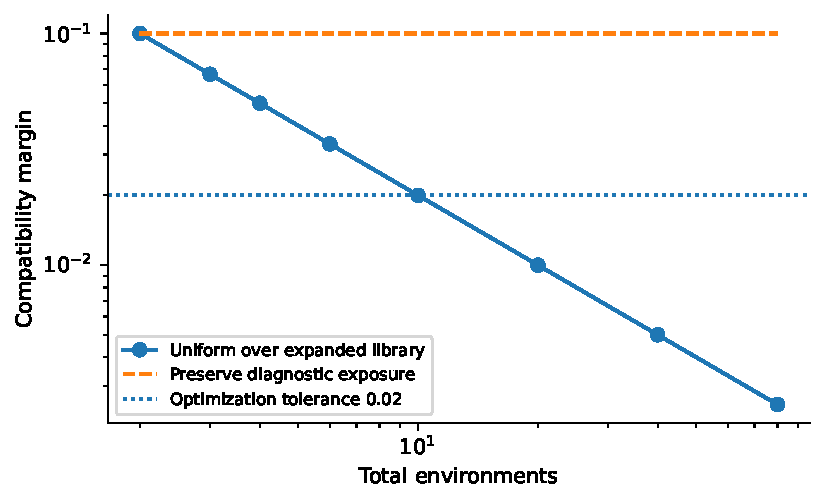
\includegraphics[width=.73\linewidth]{dilution.pdf}
\caption{Exact three-convention construction. Uniform sampling over additional neutral environments lowers the tolerance at which all near-optimal policies remain compatible. Preserving the original diagnostic exposure avoids the effect. No learned agent is involved in this figure.}
\label{fig:dilution}
\end{figure}

\section{Curriculum design with a sharp approximation guarantee}
\label{sec:algorithm}
For arbitrary finite source returns, consider $\Gam^*=\max_{\mu\in\simplex}\Gam_A(\mu;\bad)$. The objective is generally not concave. For each candidate reference $r$, define $d_{ri}(\mu)=S_r(\mu)-S_i(\mu)$ and solve
\begin{align}
 \max_{\mu,t}\quad &t \label{eq:lp}\\
 \text{subject to}\quad &\mu\in\simplex,\quad d_{ri}(\mu)\geq0\quad\forall i,\nonumber\\
 &d_{ri}(\mu)+d_{rj}(\mu)\geq t\quad\forall(i,j)\in\bad.\nonumber
\end{align}
Skip infeasible references and return the feasible solution with largest objective. Nonnegative reference gaps are essential to the approximation argument.

\begin{theorem}[Pair-sum design]\label{thm:lp}
For a nonempty bad-pair set, solving~\eqref{eq:lp} for every reference returns a curriculum $\widehat\mu$ satisfying
\begin{equation}
 \Gam_A(\widehat\mu;\bad)\geq\tfrac12\Gam^*.
\end{equation}
The factor $1/2$ is tight for this surrogate, even with two environments and three policies, and even when the selected curriculum is unique. This is not an inapproximability claim for all algorithms.
\end{theorem}
\begin{proof}
Every curriculum has a maximizing reference. For nonnegative $x,y$, $\max(x,y)\leq x+y\leq2\max(x,y)$. Hence the optimum pair-sum value $t^*$ is at least $\Gam^*$, while the returned curriculum has margin at least $t^*/2$. For sharpness use source rows $(1,0,1)$ and $(1,1/2-h,1/2-h)$, $0<h<1/2$, with only policies 1 and 2 mutually incompatible and policy 0 compatible with both. The first source alone has margin 1. The sum objective strictly prefers the second, whose margin is $1/2+h$. Taking $h\downarrow0$ proves the claim.
\end{proof}
The sharp example also explains why a compatible \emph{set} can be better than a uniquely taught reference. The exact optimum retains two good compatible policies, whereas the surrogate removes both nonreference policies but has a smaller margin.

\paragraph{A structured reduction.}
In the assignment family, the preferred convention is a source-wise optimal reference. The minimum pair-sum gap is exactly $\kappa(a;q,\eps)$: shared mistakes can be removed, and any harmful set can be split into a pair. Thus the general surrogate reduces to
\begin{equation}
 \max_{\mu,t}t\quad\text{s.t.}\quad
 \mu\in\simplex,\qquad
 \sum_e\mu_e\sum_{j\in U}D_{ej}\geq t
 \quad\forall U:q(U)>\eps.
 \label{eq:coverage-lp}
\end{equation}
This requires at most $2^d$ subset constraints rather than enumerating $K$ references and $K^2$ policy pairs for $K=2^d$. It remains exponential in $d$; there is no claim of a scalable solver for arbitrary compact classes. The positive-coverage criterion is a teaching/covering relation, while balanced partitions determine the actual tolerance.

\paragraph{Exact verification oracle.}
For small general classes we solve a mixed-integer linear program. Binary anchor variables enforce $s=\max_iS_i(\mu)$, exclusion variables form a vertex cover of $\bad$, and $t\leq s-S_i$ is enforced for excluded policies. Return bounds provide valid big-$M$ constants of 1. Appendix~\ref{app:oracle} gives the full construction; independent vertex-cover enumeration checks it on separate instances. The MILP is an oracle for validation, not the proposed scalable algorithm.

\begin{figure}[t]
\centering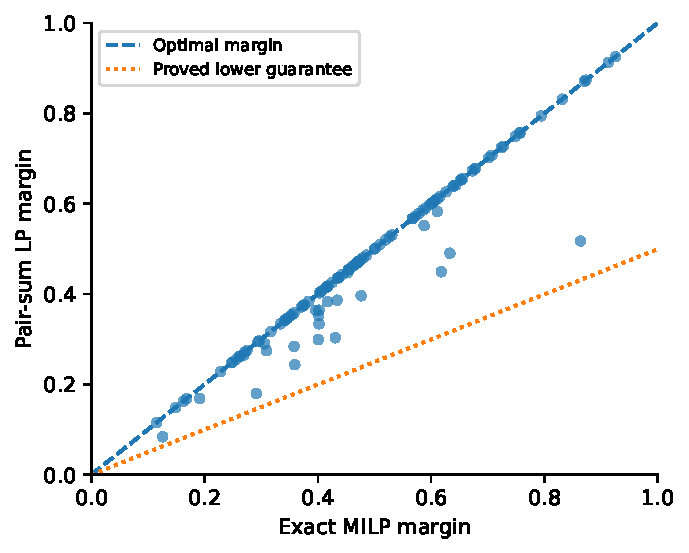
\includegraphics[width=.60\linewidth]{approximation.pdf}
\caption{General finite-class validation on 120 random return/compatibility geometries. The surrogate attains a mean $0.967$ fraction of the exact margin and matches it within $10^{-7}$ in 96 instances. A separate analytic family approaches the proved $1/2$ factor, so the favorable random ratios do not strengthen the worst-case theorem.}
\label{fig:approx}
\end{figure}

\section{Sharp certificates from finite return data}
\label{sec:statistics}
Suppose the teacher has an entry-wise confidence box $L_{ei}\leq A_{ei}\leq U_{ei}$. For a fixed curriculum define
\begin{equation}
 \ell_i(\mu)=\sum_e\mu_eL_{ei},\quad
 u_i(\mu)=\sum_e\mu_eU_{ei},\quad
 z(\mu)=\max_k\ell_k(\mu).
\end{equation}
These are intervals for individual self-play scores, not independent observations of those scores.

\begin{theorem}[Sharp rectangular certificate]\label{thm:box}
For nonempty $\bad$, the exact worst-case margin over the product box is
\begin{equation}
 \inf_{A\in[L,U]}\Gam_A(\mu;\bad)
 =\left[z(\mu)-\max_{(i,j)\in\bad}\min\{u_i(\mu),u_j(\mu)\}\right]_+
 =:\Gam_{\Box}(\mu;\bad).
 \label{eq:box}
\end{equation}
The infimum is attained. Therefore $\Gam_{\Box}>\eta$ is necessary and sufficient for every return table in the box to make every $\eta$-optimal self-play pair compatible with the specified target relation.
\end{theorem}
\noindent\emph{Interpretation.} A harmful pair can simultaneously remain near-optimal only when its smaller optimistic score approaches the largest pessimistic score available to any policy. A single closed-form calculation captures this shared competition for optimality; separate correctness checks of policies are unnecessary. The attaining matrix is explicit in Appendix~\ref{app:box}.

Sharpness is \emph{certificate-only}: it uses only the independent cell intervals. If source returns must additionally obey the shared assignment structure, the box is a relaxation and its adversarial witness need not satisfy that structure. The formula is not claimed to be the sharpest certificate using every property of a known simulator.

\begin{corollary}[Adaptive curriculum selection from fixed data]\label{cor:adaptive}
Assume the entire source box covers the true table with probability at least $1-\delta_A$. Also suppose a target lower-bound table $L^T$ satisfies $L^T_{ij}\leq T_{ij}$ simultaneously with probability at least $1-\delta_T$. Let $\bad^+=\{(i,j):L^T_{ij}<\tau\}$. Any number of curricula, chosen adaptively using these same data, satisfy all issued claims
\begin{equation}
 \Gam_{\Box}(\mu;\bad^+)>\eta
 \ \Longrightarrow\ 
 \min_{i,j\in\nearset_\eta(\mu)}T_{ij}\geq\tau
\end{equation}
with joint probability at least $1-\delta_A-\delta_T$.
\end{corollary}
There is no union bound over curricula because coverage is a single uniform event over the table. The statement does not permit unchecked optional stopping of the evaluation data or arbitrary policy-class expansion. The optimization tolerance refers to true source values; evaluating or bounding a learner's achieved gap is a separate requirement.

\paragraph{A concrete fixed-sample construction.}
With $n_{ei}$ independent bounded reward observations within each cell and predetermined counts, Hoeffding's inequality \citep{hoeffding1963} gives simultaneous radii
\begin{equation}
 b_{ei}=\sqrt{\frac{\log(2MK/\delta_A)}{2n_{ei}}}.
\end{equation}
Clip $\widehat A_{ei}\pm b_{ei}$ to $[0,1]$. Cross-cell dependence is allowed because the proof is a union bound. If a common un-clipped score radius $b$ applies to every policy,~\eqref{eq:box} reduces to $[\Gam_{\widehat A}-2b]_+$; heterogeneous intervals and clipping are handled directly rather than through this coarser expression.

\begin{proposition}[Restricted calibration lower bound]\label{prop:lower}
Consider one source, two policies with known $A_0=3/4$, and unknown Bernoulli return mean $A_1=1/2\mp h$, where $0<h\leq1/4$. Let target diagonal returns be 1, off-diagonal returns 0, $0<\tau\leq1$, and $\eta=1/4$. Any procedure that issues a valid certificate with probability at least $1-\delta$ in the safe world and issues one with probability at most $\delta$ in the unsafe world, $0<\delta<1/2$, needs
\begin{equation}
 n\geq\frac{(1-2\delta)\log((1-\delta)/\delta)}{16h^2}
\end{equation}
on a fixed sample of the unknown cell.
\end{proposition}
This is a two-world calibration bound, not a lower bound on all possible ways to learn a cooperating team. In particular, a shared fixed convention can produce agreement without learning the self-play optimum. The bound requires both certificate validity and nontrivial completeness near the optimization threshold.

\section{Experiments}
\label{sec:experiments}
All experiments are synthetic, CPU-only, and included as executable code. They use no model APIs, pretrained networks, human data, or physical robots. Scientific CSVs record fixed seeds and omit timestamps. Table values and plots are generated from the CSVs rather than transcribed manually. The reference run uses NumPy 2.3.5 and SciPy 1.17.0; its hardware-dependent timing is recorded separately.

\subsection{Exact finite checks and assumption violations}
The general design study uses 120 random tables with 3--5 sources, 4--7 policies, and random nonempty bad-pair graphs. Mean margins are $.126$ for uniform sampling, $.467$ for the LP, and $.481$ for the exact MILP. The smallest observed LP/optimal ratio is $.599$, the mean is $.967$, and 96 cases tie within $10^{-7}$. These values concern an explicitly generated finite model, not independently discovered agent conventions.

The structured study draws 300 nonnegative diagnostic matrices with 3--6 contexts and checks~\eqref{eq:balanced} against direct enumeration of every policy-pair return. Sixteen additional equal-exposure cases exhibit both unique and multiple compatible survivors. For interval sharpness, 400 heterogeneous boxes are checked against the explicit attaining construction and 4,800 interior samples. All identities agree to $10^{-9}$ in these experiments.

The scope violation adds a single policy that agrees with the optimal reference on all source environments but behaves incompatibly on the target. This is realizable when an otherwise excluded source/target flag becomes observable. Across 100 generated classes, a positive restricted-class margin becomes zero after expansion. This is not an adversarial attack on a deployed model: it is an exact counterexample to unrestricted policy-class transfer.

\subsection{Adaptive calibration is valid but conservative}
We generate 600 independent source-evaluation datasets with four sources and three policies, using $n\in\{16,64,256,1024,4096,16384\}$ samples per cell and 100 seeds for each $n$. Each dataset selects curriculum weights through the point-estimate LP. We then evaluate certificates at two tolerances, $.075$ and $.15$, giving 1,200 decisions. The target bad pair is known, while the source confidence level is $95\%$. A false certificate means that the true margin of the selected curriculum is at most the requested tolerance.

The plug-in procedure accepts 952 times, of which 211 are false; the box certificate accepts 167 times, with no false claim observed. The latter is not an empirical proof of a $5\%$ guarantee: the guarantee is Corollary~\ref{cor:adaptive}. The large abstention rate is important. A conservative interval method and an approximate design surrogate need not provide certificates at tolerances where some better-informed curriculum could succeed. Decisions sharing a dataset are not counted as independent statistical replications.

\begin{table}[t]
\centering\small\begin{tabular}{rrrrrr}
\toprule
$n$ per cell & Plug-in accepts & False & Box accepts & False & Trials \\
\midrule
16 & 199 & 77 & 0 & 0 & 200 \\
64 & 190 & 51 & 0 & 0 & 200 \\
256 & 174 & 33 & 4 & 0 & 200 \\
1024 & 165 & 32 & 40 & 0 & 200 \\
4096 & 125 & 11 & 58 & 0 & 200 \\
16384 & 99 & 7 & 65 & 0 & 200 \\
\bottomrule
\end{tabular}

\caption{Calibration totals, pooling two tolerance queries per dataset. ``False'' is measured against exact ground-truth source values. The box certifies substantially less often; this cost is not hidden by reporting only error rates.}
\label{tab:calibration}
\end{table}

\subsection{Sampled reward learning in the assignment family}
We use six contexts, diagnostic penalties
\begin{equation*}
 \Delta=(.08,.12,.18,.25,.35,.50),\qquad
 q=(.05,.08,.12,.15,.25,.35),
\end{equation*}
and preference vector $(1,0,1,1,0,1)$. Source modes either diagnose one context or are neutral. We compare libraries with zero or 24 neutral modes and target threshold $.9$. For learning, a correctly coordinated preferred assignment has Bernoulli mean $.8$; a wrong assignment has mean $.8-\Delta_j$ on diagnostic trials and $.8$ on neutral trials. Collision return is zero. These values change the common source baseline but preserve $g(b)=\sum_ja_j\1\{b_j\ne\theta_j\}$. Agents observe their context and shared reward, not the mode or preference label.

Seven curricula are compared: uniform over the entire library, uniform over diagnostic modes, diagnostic weights proportional to $1/\Delta_j$ or $1/\Delta_j^2$, concentrating on the largest-penalty context, farthest-first selection using three nuisance task features, and~\eqref{eq:coverage-lp}. The diagnostic and inverse-gap baselines have structural knowledge just as the coverage method does. Feature diversity and difficulty-only are intentionally simple controlled baselines, not stand-ins for full modern UED methods.

We train 24 independent seeds per condition at budgets of 256, 1,024, and 4,096 episodes. A parameter-space search learner explores a deterministic assignment bit during self-play and updates two empirical action values per context. Both copies execute that sampled convention during training; deterministic deployment requires no shared random coin. A second learner uses independent action sampling and a shared-logit REINFORCE update. Each receives only sampled common reward, not labels for the correct assignment. Across the two learners, seven curricula, two libraries, and three budgets there are 2,016 runs and 3,612,672 executed training episodes. Reused seeds provide matched randomness across curricula; these conditions are not 2,016 independent population samples.

Cross-play is evaluated exactly under $q$ for all ordered unequal-seed pairs. Standard errors use a delete-one-seed jackknife of this pairwise statistic, not a misleading standard error over all 552 dependent pairs. The worst observed pair is only a finite-seed statistic. Separately, the theorem covers every member of the specified finite policy class whose actual gap is at most $.8\Gam$.

\begin{table}[t]
\centering\small\begin{tabular}{lrrrr}
\toprule
Curriculum & Margin & Mean cross-play & Worst & Eligible \\
\midrule
Uniform library & 0.0040 & $0.835\,\pm\,0.028$ & 0.50 & 10/24 \\
Diagnostic uniform & 0.0200 & $0.996\,\pm\,0.004$ & 0.95 & 24/24 \\
Inverse gap & 0.0284 & $1.000\,\pm\,0.000$ & 1.00 & 24/24 \\
Inverse squared gap & 0.0070 & $1.000\,\pm\,0.000$ & 1.00 & 24/24 \\
Difficulty only & 0.0000 & $0.668\,\pm\,0.010$ & 0.35 & 0/24 \\
Coverage LP & 0.0440 & $0.976\,\pm\,0.003$ & 0.95 & 24/24 \\
Feature diversity & 0.0000 & $0.593\,\pm\,0.018$ & 0.15 & 0/24 \\
\bottomrule
\end{tabular}

\caption{Parameter-space search after 4,096 episodes with 24 neutral modes. Mean $\pm$ seed-jackknife standard error. ``Eligible'' counts seeds with true gap at most $.8\Gam$ when $\Gam>0$; zero-margin curricula certify none. The coverage LP optimizes guaranteed tolerance, not mean cross-play, and is not uniformly best empirically.}
\label{tab:learning}
\end{table}

The coverage LP ignores the lowest-target-mass context and gives five retained contexts equal diagnostic exposure. Its margin $.04396$ exceeds $.02000$ for diagnostic-uniform and $.00400$ for the full uniform library. At 4,096 search episodes, all 24 coverage-trained policies have zero training gap yet retain two compatible conventions, because behavior on the ignored context is unconstrained. Their mean cross-play is $.9755$ and worst cross-play is $.95$, above the required $.9$. The inverse-gap rules instead reach a common convention and mean 1.000. This is a real tradeoff, not an empirical win for our method on every metric.

\begin{figure}[t]
\centering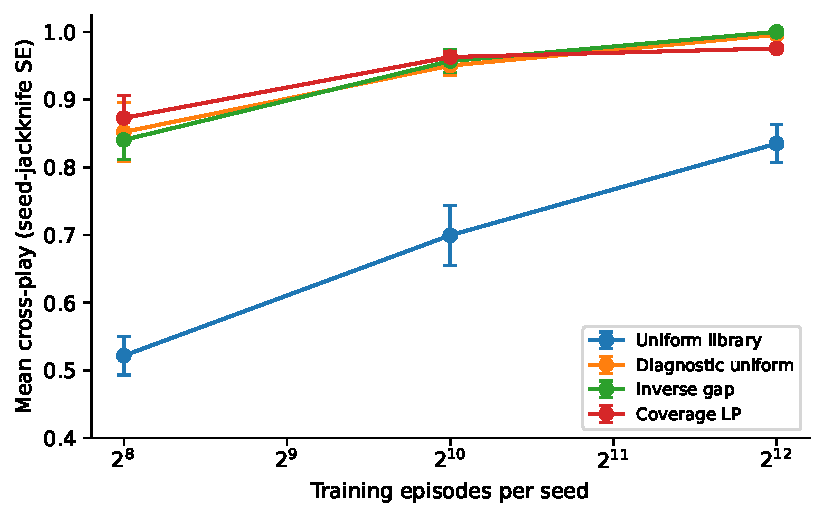
\includegraphics[width=.73\linewidth]{learning_search.pdf}
\caption{Sampled-reward parameter-space search with 24 neutral environments, 24 seeds per point. Diagnostic exposure improves learned cooperation relative to diluted uniform sampling; a simpler inverse-gap curriculum can outperform the margin optimizer on mean target return. Error bars are seed-jackknife standard errors.}
\label{fig:search}
\end{figure}

\subsection{A positive margin does not remove local optima}
\begin{proposition}[Local-optimization obstruction]\label{prop:local}
For one context with independent action sampling and $p$ the probability of the wrong convention bit, let $r_0>r_1>0$ be preferred and nonpreferred coordinated returns. The self-play objective is
\begin{equation}
 f(p)=r_0(1-p)^2+r_1p^2.
\end{equation}
Both deterministic boundaries are strict local maxima on $[0,1]$, separated by a minimum at $p=r_0/(r_0+r_1)$. With independent parameters across $d$ positively weighted contexts, every deterministic convention is a local maximum, although only preferred conventions are globally optimal when every context is diagnostic.
\end{proposition}
Independent-action policy gradient is consistent with this obstruction. For the coverage curriculum at 4,096 episodes, mean cross-play is $.5765$, the worst observed pair has return 0, and only 2 of 24 seeds satisfy the theoretical gap threshold. Their mutual target return is at least $.95$, but such a small eligible subset does not make the full team reliable. The theory predicts a guarantee \emph{after} near-optimality, not convergence to it. Search and REINFORCE deliberately use different exploration mechanisms; their comparison diagnoses optimization, not an across-algorithm superiority claim.

\begin{figure}[t]
\centering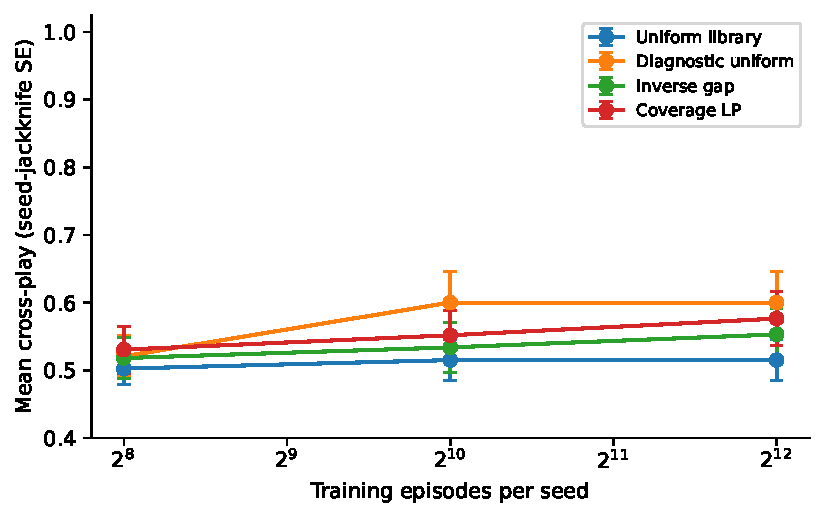
\includegraphics[width=.73\linewidth]{learning_reinforce.pdf}
\caption{Independent-action self-play policy gradient does not generally reach the near-optimal set required by the certificate. Diagnostic weighting alone is insufficient. These negative results and all seed-level returns are retained in the release.}
\label{fig:reinforce}
\end{figure}

\section{Limitations and implications}
The guarantee concerns pairwise cooperation within a finite, fixed policy class. A certificate for a restricted library does not automatically cover novel neural policies. Source/target flags, unseen observations, memory, or arbitrary parameter sharing can invalidate the structured assignment model. The target distribution and the relation between its reward and source dynamics are specified; the work does not establish unrestricted domain generalization. There is no sequential credit assignment, physical contact, language communication, or human modeling in the experiment.

Curriculum optimization requires source diagnostics or a return table, and an exact or conservative target incompatibility relation. The finite-data certificate does not make those inputs free. Its intervals can be highly conservative and its sharpness ignores additional simulator constraints. The sample lower bound is intentionally narrow. The LP's approximation concerns margin, not training sample complexity, number of source modes, actual learner convergence, or target-return optimality. The learned results show these quantities can disagree.

The connection to teaching and version-space diameter is substantive. A convincing broader follow-up would need either more general structural results or evaluation where discovering diagnostics is itself difficult. The present contribution is a precise diagnostic-exposure theory with falsifiable assumptions and reproducible small validation, not evidence that the proposed curriculum is a universal multi-agent training method.

\section{Conclusion}
Training environments teach transferable cooperation only when their weighted reward differences remove harmful combinations of plausible learned conventions. In a restricted assignment family, an exact balanced-coverage formula identifies both invisible target mass and the two-learner error budget that exposure must overcome. A sharp factor-two design surrogate and an exact interval certificate make the finite-class formulation constructive. Controlled experiments verify these relations while exposing two important limits: optimizing the certificate need not optimize average cross-play, and diagnostic information does not solve nonconvex self-play optimization. These distinctions provide a concrete basis for deciding what an environment library can teach, what evidence can certify, and what a learner still must achieve.

\paragraph{Reproducibility statement.}
The accompanying repository contains the simulator, LP and MILP solvers, interval witnesses, both sampled-reward learners, fixed-seed scientific CSVs, table and figure generation, and unit tests. Commands and every hyperparameter are in Appendix~\ref{app:reproduction}. The manuscript is a research draft with self-checked proofs; independent mathematical and novelty review has not been completed.

\bibliographystyle{plainnat}
\bibliography{references}
\clearpage\appendix

\section{Proofs for the assignment family}\label{app:balanced}
\subsection{Balanced coverage and sharp constants}
\begin{proof}[Proof of Theorem~\ref{thm:balanced}]
Relabel the preferred convention as $\theta=0$. It has value 1 in every source, so the gap of any convention $b$ is $a(B)$ for $B=\{j:b_j=1\}$. For a second convention with error set $C$, the target loss is $q(B\triangle C)$. If this pair is bad, let $U=B\triangle C$, $V=B\setminus C$, and $Z=C\setminus B$. Then $V,Z$ are disjoint, $V\cup Z=U$, and
\begin{equation*}
 a(V)\leq a(B),\qquad a(Z)\leq a(C).
\end{equation*}
The two conventions with error sets $V,Z$ are still bad and have no larger maximum gap. Hence restricting the minimizing pair to disjoint error sets loses nothing. Conversely, every $U$ with $q(U)>\eps$ and every partition $V,U\setminus V$ specifies a bad pair in the class. Taking their maximum gaps gives~\eqref{eq:balanced} and the budget equivalence.

For each partition, $\max\{a(V),a(U\setminus V)\}\geq a(U)/2$. Minimizing gives $\Gam\geq\kappa/2$. Choosing $V=U$ gives a feasible value $a(U)$, and then minimizing over $U$ gives $\Gam\leq\kappa$.

The upper constant is attained for $d=1$, $q_1=1$, any $\eps<1$, and positive exposure $a_1$: every harmful pair differs on that coordinate and the larger gap is $a_1$. For the lower constant, set $d=2$, $q=(1/2,1/2)$, $\eps=3/4$, and $a=(s,s)$ with $0<s\leq1/2$. The only harmful coordinate set is $\{1,2\}$; splitting it into singletons gives $\Gam=s=\kappa/2$. The values are realizable with a diagnostic matrix of nonnegative entries and row sum at most 1.
\end{proof}

\subsection{Invisible contexts and support restrictions}
\begin{proof}[Proof of Corollary~\ref{cor:observable}]
If $q(Z)>\eps$, choose the preferred convention and the convention that flips exactly $Z$. Their source errors have zero exposure under every curriculum, so both are exact maximizers and their target pair is bad. Thus the margin is zero.

Conversely, suppose $q(Z)\leq\eps$. Give every admissible source positive weight. Every coordinate outside $Z$ then has strictly positive exposure. A harmful set $U$ cannot be contained in $Z$, so $a(U)>0$. There are finitely many subsets, hence $\kappa=\min_{U:q(U)>\eps}a(U)>0$. Theorem~\ref{thm:balanced} gives $\Gam\geq\kappa/2>0$. Restricting the admissible modes to a prescribed support $S$ gives the second statement by the same argument, with positive weights on $S$.
\end{proof}
This proof establishes existence of \emph{some} positive tolerance. It does not bound that tolerance uniformly over arbitrarily small nonzero penalties.

\subsection{Neutral exposure and curriculum expansion}
\begin{proof}[Proof of Proposition~\ref{prop:dilution}]
For every policy $i$, the new score is $S'_i=pS_i+c$, where $c$ aggregates all neutral-mode baselines and is independent of $i$. Therefore
\begin{equation*}
 \max_kS'_k-S'_i=p(\max_kS_k-S_i).
\end{equation*}
For nonempty $\bad$, both maxima within pairs and the minimum across pairs commute with multiplying by $p\geq0$. This gives $\Gam'=p\Gam$. Uniform sampling over $M+N$ modes gives $p=M/(M+N)$. By contrast, setting new-mode weights to zero embeds the original feasible simplex in the expanded one, so the optimized margin cannot decrease.
\end{proof}

\subsection{Why unobserved behavior cannot be certified}
Suppose the policy class is enlarged to include $\pi'$ that matches an optimal reference on every source but changes behavior on a target-only observation. If $T(\pi',\pi_r)<\tau$, both are zero-gap policies under every curriculum for which $r$ is optimal. Their bad edge has maximum gap zero, so no positive certificate is possible. In the source-flag construction, $\pi'$ can match the source optimum under every source mixture, making this obstruction universal. This proves the class-expansion experiment algebraically, without relying on training outcomes.

\section{Optimization and the exact oracle}\label{app:oracle}
\subsection{Why all references are needed}
A return-maximizing policy can change as $\mu$ changes. Fixing an arbitrary reference need not cover the optimum of~\eqref{eq:margin}. Let
\begin{equation*}
 \mathcal M_r=\{\mu:S_r(\mu)\geq S_i(\mu)\ \forall i\}.
\end{equation*}
These closed polytopes cover the simplex. On $\mathcal M_r$, all $d_{ri}$ equal the true nonnegative gaps. The minimum pair-sum objective is at least the margin and at most twice the margin pointwise. Taking the best reference yields Theorem~\ref{thm:lp}. All maxima exist by compactness and continuity for a nonempty finite bad set.

The sharp three-policy example has target matrix
\begin{equation*}
 T=\begin{pmatrix}1&1&1\\1&1&0\\1&0&1\end{pmatrix},\qquad 0<\tau\leq1.
\end{equation*}
For weight $x$ on the first source, policy 0 is always optimal, and the two other gaps are
\begin{equation*}
 g_1=x+(1-x)(1/2+h),\quad g_2=(1-x)(1/2+h).
\end{equation*}
Their sum is $1+2h-2hx$, uniquely maximized at $x=0$, whereas their maximum is maximized at $x=1$ with value 1. At $x=1$, policies 0 and 2 tie at the optimal source score and are compatible. This verifies both the strict surrogate preference and the claimed harmless nonuniqueness.

\subsection{Structured pair-sum reduction}
A pair with error sets $B,C$ has gap sum
\begin{equation*}
 a(B)+a(C)=a(B\triangle C)+2a(B\cap C).
\end{equation*}
For a bad pair, the first term is at least $\kappa$. Removing the intersection yields a valid pair with sum exactly $a(B\triangle C)$. Every harmful set is attainable, for example by pairing its error convention with the preferred convention. Therefore the minimum sum is exactly $\kappa$, which is linear in $\mu$ for each subset constraint and gives~\eqref{eq:coverage-lp}.

\subsection{A mixed-integer formulation}
Introduce continuous variables $\mu\in\Delta_M$, $s,t\in[0,1]$, exclusion binaries $y_i$, and anchor binaries $z_i$. Solve
\begin{align*}
 \max\quad &t\\
 \text{s.t.}\quad &s\geq S_i(\mu),\quad s\leq S_i(\mu)+1-z_i&&\forall i,\\
 &\sum_i z_i=1,\\
 &t\leq s-S_i(\mu)+1-y_i&&\forall i,\\
 &y_i+y_j\geq1&&(i,j)\in\bad.
\end{align*}
For a diagonal edge the last inequality forces its binary to 1. An active anchor makes $s$ equal to an attained maximum score. For every bad edge at least one endpoint is excluded, and its gap is at least $t$, so any feasible solution has $t\leq\Gam$. Conversely, given $\mu$, choose an optimal anchor and let $y_i=1$ whenever $g_i\geq\Gam(\mu)$. These vertices cover every bad edge, making $t=\Gam(\mu)$ feasible. Bounds in $[0,1]$ make all relaxed constraints valid. Thus the MILP optimum equals $\Gam^*$.

The implementation recomputes the returned margin from its weights and checks agreement with the optimization objective. HiGHS feasibility tolerances are tightened to $10^{-9}$, since default integer feasibility can otherwise slightly overstate the margin. Separate tests enumerate vertex covers and solve their reference-conditioned LPs, providing an implementation-independent small-instance check.

\section{Statistical proofs}\label{app:box}
\subsection{Proof and construction for the rectangular certificate}
\begin{proof}[Proof of Theorem~\ref{thm:box}]
For fixed $\mu$, the score of policy $i$ ranges over the entire interval $[\ell_i,u_i]$. Indeed, the linear image of its source interval product is this interval; different policies use different columns, so these score intervals vary independently over the product box.

Fix a bad pair $(i,j)$ and write $m=\min(u_i,u_j)$ and $z=\max_k\ell_k$. For any feasible score vector $s$, its maximum $s_*\geq z$, and $\min(s_i,s_j)\leq m$. The larger of the two gaps is
\begin{equation*}
 \max(s_*-s_i,s_*-s_j)=s_*-\min(s_i,s_j)\geq[z-m]_+.
\end{equation*}
This bound is attainable. Set $s_k=\ell_k$ for every other coordinate, and set
\begin{equation*}
 s_i=\max(\ell_i,m),\qquad s_j=\max(\ell_j,m).
\end{equation*}
These values are within their intervals; at least the endpoint with smaller upper limit has score exactly $m$. Thus their minimum is $m$ and the maximum overall score is $\max(z,m)$. The same construction works for $i=j$.

To realize the chosen vector by a source table, when $u_k>\ell_k$ define
\begin{equation*}
 \lambda_k=\frac{s_k-\ell_k}{u_k-\ell_k},\qquad
 A_{ek}=L_{ek}+\lambda_k(U_{ek}-L_{ek}).
\end{equation*}
When $u_k=\ell_k$, simply use the lower column. This construction remains valid when some source weights are zero.

Finally, the minimum over finitely many pairs commutes with the infimum over the box: both equal the joint infimum over a table and an edge. Minimizing $[z-\min(u_i,u_j)]_+$ yields~\eqref{eq:box}, and the edge maximizing its smaller upper limit supplies the witness. Compactness and the explicit construction establish attainment, including the zero case. Lemma~\ref{lem:margin} then gives the necessary-and-sufficient robust statement.
\end{proof}

\subsection{Adaptive selection and unknown target values}
\begin{proof}[Proof of Corollary~\ref{cor:adaptive}]
On the simultaneous source-coverage event, the true return table is in the box, so Theorem~\ref{thm:box} lower-bounds its margin for \emph{every} curriculum, without restricting how the weights were selected. On the simultaneous target event, a truly bad pair satisfies $T_{ij}<\tau$ and hence $L^T_{ij}\leq T_{ij}<\tau$, placing it in $\bad^+$. Certifying against this superset is conservative. Applying Lemma~\ref{lem:margin} on the intersection of the two events proves every issued implication. A union bound on their failures gives $\delta_A+\delta_T$; independence is not needed.
\end{proof}
For empirical means from predetermined bounded samples, each Hoeffding interval fails with probability at most $\delta_A/(MK)$. A union bound gives the simultaneous source event. The mathematical guarantee is exact conditional on that event, whereas the observed absence of false claims in the synthetic study is a separate empirical check.

\subsection{Two-world lower bound}
\begin{proof}[Proof of Proposition~\ref{prop:lower}]
In the safe world, policy 1 has source mean $p=1/2-h$, so the gap between the policies is $1/4+h>\eta$. Only policy 0 can remain $\eta$-optimal and a certificate is true. In the unsafe world, the mean is $q=1/2+h$, so both policies are $\eta$-optimal and their target pair fails. Let $C$ be the event that the procedure issues the certificate. The assumed error and power guarantees imply $P(C)\geq1-\delta$ and $Q(C)\leq\delta$.

Data processing of relative entropy under the binary map $\1_C$ gives
\begin{equation*}
 n\,\kl(p,q)\geq\kl(P(C),Q(C))\geq\kl(1-\delta,\delta)
 =(1-2\delta)\log\frac{1-\delta}{\delta}.
\end{equation*}
Independent auxiliary randomness of the procedure contributes no relative entropy. For $0<h\leq1/4$,
\begin{equation*}
 \kl(1/2-h,1/2+h)=2h\log\frac{1+2h}{1-2h}
 \leq 2h\frac{4h}{1-2h}\leq16h^2.
\end{equation*}
Combining proves the stated bound. A procedure that always abstains is excluded by the safe-world completeness requirement. A procedure whose sole objective is agreement rather than near-optimal-set certification need not face this test.
\end{proof}

\section{Optimization obstruction and experimental details}\label{app:reproduction}
\subsection{Independent-action self-play}
\begin{proof}[Proof of Proposition~\ref{prop:local}]
Independently sampled convention bits match at the preferred assignment with probability $(1-p)^2$ and at the wrong assignment with probability $p^2$; the remaining probability produces zero reward. Differentiation gives
\begin{equation*}
 f'(p)=-2r_0+2(r_0+r_1)p,\qquad f''(p)=2(r_0+r_1)>0.
\end{equation*}
Thus the interior stationary point is a strict minimum, $f'(0)<0$, and $f'(1)>0$. Moving into the interval from either boundary decreases value, so both boundaries are strict local maxima. A positively weighted sum across contexts has the same property independently in each coordinate. The wrong boundary is globally worse by $r_0-r_1$, but local improvement cannot escape it without first decreasing return.
\end{proof}
For the noisy assignment experiment, source mixing gives $r_{0j}=.8\Pr(J=j)$ and $r_{1j}=r_{0j}-a_j$ in the weighted objective. Whenever both are positive, changing curriculum weights does not remove the two boundary optima. Contexts assigned zero probability remain entirely unconstrained.

\subsection{Algorithms and fixed settings}
The search learner keeps two empirical means per context, initialized at $.5$ with pseudo-count 1. Each observed context uses $\epsilon$-greedy exploration with fixed $\epsilon=.2$; ties use private seeded randomness. It samples one deterministic role-conditioned convention for both copies in that training trial, receives the shared Bernoulli reward, and updates only the sampled option. This is parameter-space policy search, not independent decentralized action exploration. Final deployment chooses the larger empirical mean; remaining ties use a private seeded default.

The independent-action learner maintains one logit per context, initialized independently from $\mathcal N(0,1.2^2)$. Both roles sample convention bits independently from its sigmoid. A shared scalar reward and a context-dependent running baseline produce gradient $(R-B)(a_0+a_1-2p)$, with step size $.12$, baseline update $.05(R-B)$, and logits clipped to $[-10,10]$. Final policies are greedified at zero logit. The finite-class certificate concerns these deterministic deployed policies, not the stochastic training policy. Budgets share the same initializations and random-stream prefixes; methods reuse seed-indexed randomness without sharing information between independently trained seeds.

All curriculum methods receive the same per-seed episode budgets. The teacher's computational budget and prior structural knowledge are not counted as learner episodes. The inverse-gap and inverse-squared-gap baselines place no weight on neutral modes. The difficulty baseline chooses the largest diagnostic penalty. The feature baseline starts at the first mode and greedily selects four modes by Euclidean farthest-first distance on $(\operatorname{linspace}(-1,1),\cos e,\sin(1.7e))$. These are nuisance features on purpose: this baseline tests whether irrelevant variation can substitute for diagnostics, not whether every reasonable diversity representation fails.

\subsection{Finite-generation protocols}
The 120 general geometries use independent uniform source returns, dimensions cycling through 3--5 environments and 4--7 policies, and off-diagonal bad edges sampled at probability $.5$ with a fixed fallback edge if empty. They are realizable as finite cooperative source and target payoff tables but need not obey the structured assignment factorization.

For structured checks, rows of $D$ are Dirichlet context weights multiplied by independent penalties in $[.05,.6]$. Curricula and target weights are Dirichlet, and tolerances cycle through $.071,.217,.413$. The 400 interval geometries alternate wider boxes and boxes narrowed by a factor of 50; some include a diagonal bad pair. Each has an explicit adversarial witness and 12 interior checks. Counts in the calibration study are predetermined, and Bernoulli sufficient statistics are sampled directly using a binomial generator. Those are calibration simulations, not additional executed policy rollouts.

Exact target matrices are computed from $q$ and the deployed bits. Thus evaluation uses no finite target sample and does not conflate target Monte Carlo noise with cross-seed variation. Physical scale changes are analytically invariant under the normalized reward; we do not count them as independent tests of generalization. A wider task family with previously unseen meaningful features remains future validation.

\subsection{Dependence-aware empirical uncertainty}
For $n=24$ learned seeds, let
\begin{equation*}
 \widehat U=\frac{1}{n(n-1)}\sum_{i\ne j}T(b_i,b_j).
\end{equation*}
Compute $\widehat U_{-i}$ with seed $i$ removed and jackknife pseudovalues $v_i=n\widehat U-(n-1)\widehat U_{-i}$. The reported standard error is the sample standard deviation of the pseudovalues divided by $\sqrt n$. No significance claims are based on treating pairs as independent. Identical curricula in the zero-neutral and 24-neutral libraries intentionally produce identical trajectories under matched random streams.

\subsection{Reproduction commands and checks}
From the repository root, with Python 3.11 or newer:
\begin{verbatim}
python -m pip install -e '.[test]'
python -m pytest -q
OPENBLAS_NUM_THREADS=1 OMP_NUM_THREADS=1 \
    python experiments/run_all.py
python experiments/report.py
cd paper
pdflatex -interaction=nonstopmode -halt-on-error main.tex
bibtex main
pdflatex -interaction=nonstopmode -halt-on-error main.tex
pdflatex -interaction=nonstopmode -halt-on-error main.tex
\end{verbatim}
The reference execution uses Python 3.13.5. The test suite checks the strict near-optimal boundary, loops and empty graphs, LP approximation, tight examples, station returns, structured/direct agreement, box witnesses, dilution, policy-class expansion, learner seed batching, and the calibration lower-bound constant. An independent vertex-cover enumeration checks the MILP separately from the surrogate. Scientific CSVs can be regenerated into a separate directory and compared; the run metadata file is intentionally not byte-identical because it contains runtime and platform information. Numerical comparisons use tolerances rather than claiming formal machine verification of the proofs.

\section{Claim audit}
The pair-exclusion characterization is elementary. The nontrivial proposed research content is its constructive specialization to balanced diagnostic exposure, the accompanying attainable design and interval guarantees, and the demonstrated separation between diagnostic adequacy and self-play optimization. All theorems in this draft have explicit proofs; their status is self-checked, not independently peer reviewed. The approximation factor is tight for the stated surrogate only. The interval formula is sharp for the stated rectangular information set only. The lower bound is for a fixed two-world certificate-testing problem only. The learned study is one deliberately restricted contextual task family, and the best empirical method depends on the metric. These limits should remain visible in any subsequent submission rather than being replaced by claims of general-purpose cooperative intelligence.
\end{document}
